\chapter{Products and Quotients of Groups}
\label{chapter:products_quotients}
\thispagestyle{empty}

\begin{section}{Products of Groups}

In this section, we will discuss a method for using existing groups as building blocks to form new groups.

Suppose $(G,*)$ and $(H,\circ)$ are two groups.  Recall that the Cartesian product of $G$ and $H$ is define to be
\[
G\times H=\{(g,h):g\in G,h\in H\}
\]
For more information on Cartesian products, see Definition~\ref{def:cartesian_product}.  Using the binary operations for the groups $G$ and $H$, we can define a binary operation on the set $G\times H$.  Define $\star$ on $G\times H$ via
\[
(g_1,h_1)\star(g_2,h_2)=(g_1*g_2,h_1\circ h_2).
\]
This looks fancier than it is.  We're just doing the operation of each group in the appropriate component.  It turns out that $(G\times H,\star)$ is a group.

\begin{theorem}
Suppose $(G,*)$ and $(H,\circ)$ are two groups, where $e$ and $e'$ are the identity elements of $G$ and $H$, respectively.   Then $(G\times H,\star)$ is a group, where $\star$ is defined as above.  Moreover, $(e,e')$ is the identity of $G\times H$ and the inverse of $(g,h)\in G\times H$ is given by $(g,h)^{-1}=(g^{-1},h^{-1})$.
\end{theorem}

We refer to $G\times H$ as the \textbf{direct product} of the groups $G$ and $H$.  Note that we abbreviate $(g_1,h_1)\star(g_2,h_2)=(g_1*g_2,h_1\circ h_2)$ by $(g_1,h_1)(g_2,h_2)=(g_1 g_2,h_1 h_2)$.

There's no reason we can't do this for more than two groups.  If $A_1, A_2, \ldots, A_n$ is a collection of sets, we define
\[
\prod_{i=1}^nA_i:=A_1\times A_2\times \cdots \times A_n.
\]
Each element of $\prod_{i=1}^nA_i$ is of the form $(a_1,a_2,\ldots, a_n)$, where $a_i\in A_i$.

\begin{theorem}
Let $G_1, G_2,\ldots, G_n$ be groups.  For $(a_1,a_2, \ldots, a_n), (b_1,b_2,\ldots, b_n)\in \prod_{i=1}^nG_i$, define
\[
(a_1,a_2, \ldots, a_n)(b_1,b_2,\ldots, b_n)=(a_1b_1,a_2b_2,\ldots, a_nb_n).
\]
Then $\prod_{i=1}^nG_i$, the \textbf{direct product} of $G_i$, is a group under this binary operation.
\end{theorem}

Note that each $G_i$ above is called a \textbf{factor} of the direct product.  One way to think about direct products is that we can navigate the product by navigating each factor simultaneously but independently. 

\begin{theorem}
Let $G_1, G_2,\ldots, G_n$ be finite groups.  Then
\[
|G_1\times G_2\times \cdots \times G_n|=|G_1|\cdot|G_2|\cdots |G_n|.
\]
\end{theorem}

\begin{theorem}
Let $G_1, G_2,\ldots, G_n$ be groups.  Then $|G_1\times G_2\times \cdots \times G_n|$ is infinite if and only if at least one $|G_i|$ is infinite.
\end{theorem}


The following theorem should be clear.

\begin{theorem}\label{thm:product_abelian_groups}
Let $G_1, G_2,\ldots, G_n$ be groups.  Then $\prod_{i=1}^nG_i$ is abelian if and only if each $G_i$ is abelian.
\end{theorem}

If each $G_i$ is abelian, then we may use additive notation.  For example, consider $\mathbb{Z}_2\times \mathbb{Z}_3$ under the operation of addition mod 2 in  the first component and addition mod 3 in the second component.  Then
\[
\mathbb{Z}_2\times \mathbb{Z}_3=\{(0,0),(0,1),(0,2),(1,0),(1,1),(1,2)\}.
\]
Since $\mathbb{Z}_2$ and $\mathbb{Z}_3$ are cyclic, both groups are abelian, and hence $\mathbb{Z}_2\times \mathbb{Z}_3$ is abelian.  In this case, we will use addition notation in $\mathbb{Z}_2\times \mathbb{Z}_3$.  For example,
\[
(0,1)+(1,2)=(1,0)
\]
and
\[
(1,2)+(0,2)=(1,1).
\]

There is a very natural generating set for $\mathbb{Z}_2\times \mathbb{Z}_3$, namely, $\{(1,0),(0,1)\}$ since $1\in \mathbb{Z}_2$ and $1\in \mathbb{Z}_3$ generate $\mathbb{Z}_2$ and $\mathbb{Z}_3$, respectively.

\begin{exercise}
Draw the Cayley diagram for $\mathbb{Z}_2\times \mathbb{Z}_3$ using $\{(1,0),(0,1)\}$ as the generating set.  Do you see a subgroup of $\mathbb{Z}_2\times \mathbb{Z}_3$ isomorphic to $\mathbb{Z}_2$ in the Cayley diagram?  What is this subgroup?  How about a subgroup isomorphic to $\mathbb{Z}_3$?
\end{exercise}

\begin{exercise}
Prove that $\mathbb{Z}_2\times \mathbb{Z}_3$ is a cyclic group of order 6 and hence isomorphic to $R_6$.  
\end{exercise}

Let's play with a few more examples.

\begin{exercise}
Consider $\mathbb{Z}_2\times \mathbb{Z}_2$ under the operation of addition mod 2 in each component.  Find a generating set for $\mathbb{Z}_2\times \mathbb{Z}_2$ and then create a Cayley diagram for this group.  What well-known group is $\mathbb{Z}_2\times \mathbb{Z}_2$ isomorphic to?
\end{exercise}

Consider the similarities and differences between $\mathbb{Z}_2\times \mathbb{Z}_3$ and $\mathbb{Z}_2\times \mathbb{Z}_2$.  Both groups are abelian by Theorem~\ref{thm:product_abelian_groups}, but only the former is cyclic.  Here's another exercise.

\begin{problem}
Consider $\mathbb{Z}_2\times \mathbb{Z}_4$ under the operation of addition mod 2 in the first component and addition mod 4 in the second component. 
\begin{enumerate}
\item[(a)] Using $\{(1,0),(0,1)\}$ as the generating set, draw the Cayley diagram for $\mathbb{Z}_2\times \mathbb{Z}_4$.
\item[(b)] Draw the subgroup lattice for $\mathbb{Z}_2\times \mathbb{Z}_4$.
\item[(c)] Show that $\mathbb{Z}_2\times \mathbb{Z}_4$ is abelian but not cyclic.
\item[(d)] Argue that $\mathbb{Z}_2\times \mathbb{Z}_4$ cannot be isomorphic to any of $D_4$, $R_8$, and $Q_8$.
\end{enumerate}
\end{problem}

The upshot of the previous problem is that there are at least 4 groups of order 8 up to isomorphism.  We'll show later that there are actually (at least) 5. The previous exercises have hinted at the following theorem.

\begin{theorem}
The group $\mathbb{Z}_m\times \mathbb{Z}_n$ is cyclic if and only if $m$ and $n$ are relatively prime.
\end{theorem}

\begin{corollary}
The group $\mathbb{Z}_m\times \mathbb{Z}_n$ is isomorphic to $\mathbb{Z}_{mn}$ if and only if $m$ and $n$ are relatively prime.
\end{corollary}

The previous results can be extended to more than two factors.

\begin{theorem}
The group $\prod_{i=1}^n \mathbb{Z}_{m_i}$ is cyclic and isomorphic to $\mathbb{Z}_{m_1m_2\cdots m_n}$ if and only if any pair from the collection $\{m_1,m_2,\ldots, m_n\}$ is relatively prime.
\end{theorem}

\begin{exercise}
Determine whether each of the following groups is cyclic.
\begin{enumerate}
\item[(a)] $\mathbb{Z}_7\times \mathbb{Z}_8$
\item[(b)] $\mathbb{Z}_7\times \mathbb{Z}_7$
\item[(c)] $\mathbb{Z}_2\times \mathbb{Z}_7\times \mathbb{Z}_8$
\item[(d)] $\mathbb{Z}_5\times \mathbb{Z}_7\times \mathbb{Z}_8$
\end{enumerate}
\end{exercise}

\begin{theorem}
Suppose $n=p_1^{n_1}p_2^{n_2}\cdots p_r^{n_r}$, where each $p_i$ is a distinct prime number.  Then
\[
\mathbb{Z}_n\cong \mathbb{Z}_{p_1^{n_1}}\times \mathbb{Z}_{p_2^{n_2}}\times \cdots \times \mathbb{Z}_{p_r^{n_r}}.
\]
\end{theorem}

\begin{theorem}
Suppose $G$ and $H$ are two groups.  Then $G\times H\cong H\times G$.
\end{theorem}

The next theorem tells us how to compute the order of an element in a direct product of groups.

\begin{theorem}
Suppose $G_1, G_2,\ldots, G_n$ are groups and let $(g_1,g_2,\ldots, g_n)\in \prod_{i=1}^nG_i$.  If $|a_i|=r_i<\infty$, then $|(a_1,a_2,\ldots, a_n)|=\lcm(r_1,r_2,\ldots,r_n)$.
\end{theorem}

\begin{exercise}
Find the order of each of the following elements.
\begin{enumerate}
\item[(a)] $(6,5)\in\mathbb{Z}_{12}\times \mathbb{Z}_7$.
\item[(b)] $(r,i)\in D_3\times Q_8$.
\item[(c)] $((1,2)(3,4),3)\in S_4\times \mathbb{Z}_{15}$.
\end{enumerate}
\end{exercise}

\begin{exercise}
Find the largest possible order in each of the following groups.
\begin{enumerate}
\item[(a)] $\mathbb{Z}_6\times \mathbb{Z}_8$
\item[(b)] $\mathbb{Z}_9\times \mathbb{Z}_{12}$
\item[(c)] $\mathbb{Z}_4\times \mathbb{Z}_{18}\times \mathbb{Z}_{15}$
\end{enumerate}
\end{exercise}

\begin{theorem}
Suppose $G_1$ and $G_2$ are groups such that $H_1\leq G_1$ and $H_2\leq G_2$.  Then $H_1\times H_2\leq G_1\times G_2$.
\end{theorem}

However, not every subgroup of a direct product has the form above. 

\begin{problem}
Find an example that illustrates that not every subgroup of a direct product is the direct product of subgroups of the factors.
\end{problem}

\begin{theorem}
Suppose $G_1$ and $G_2$ are groups with identities $e_1$ and $e_2$, respectively.  Then $\{e_1\}\times G_2\trianglelefteq G_1\times G_2$ and $G_1\times \{e_2\}\trianglelefteq G_1\times G_2$.
\end{theorem}

\begin{theorem}
Suppose $G_1$ and $G_2$ are groups with identities $e_1$ and $e_2$, respectively.  Then $\{e_1\}\times G_2\cong G_2$ and $G_1\times \{e_2\}\cong G_1$.
\end{theorem}

The next theorem describes precisely the structure of finite abelian groups.  We will omit its proof, but allow ourselves to utilize it as needed.

\begin{theorem}[Fundamental Theorem of Finitely Generated Abelian Groups]
Every finitely generated abelian group $G$ is isomorphic to a direct product of cyclic groups of the form
\[
\mathbb{Z}_{p_1^{n_1}}\times \mathbb{Z}_{p_2^{n_2}}\times \cdots \times \mathbb{Z}_{p_r^{n_r}}\times \mathbb{Z}^k,
\]
where each $p_i$ is a prime number (not necessarily distinct).  The product is unique up to rearrangement of the factors.
\end{theorem}

Note that the number $k$ is called the \textbf{Betti number}.  A  finitely generated abelian group is finite if and only if the Betti number is 0.

\begin{exercise}
Find all abelian groups up to isomorphism of order 8.  How many different groups up to isomorphism (both abelian and non-abelian) have we seen and what are they?
\end{exercise}

\begin{exercise}
Find all abelian groups up to isomorphism for each of the following orders.
\begin{enumerate}
\item[(a)] 16
\item[(b)] 12
\item[(c)] 25
\item[(d)] 30
\item[(e)] 60
\end{enumerate}
\end{exercise}

\end{section}

\begin{section}{Quotients of Groups}

In this previous section, we discussed a method for constructing ``larger" groups from ``smaller" groups using a direct product construction.  In this section, we will in some sense do the opposite.

Problem~\ref{prob:checkerboard} hinted that if $H\leq G$ and we arrange the Cayley table according to the left cosets of $H$, then the group table will have checkerboard pattern if and only if $H$ is normal in G (i.e., the left and right cosets of $H$ are the same).  For example, see the colored table prior to Exercise~\ref{exer:normal_in_D3} versus the ones you created in Exercises~\ref{exer:normal_in_D3}, \ref{exer:normal_in_Q8}.  If we have the checkerboard pattern in the group table that arises from a normal subgroup, then by ``gluing together" the colored blocks, we obtain a group table for a smaller group that has the cosets as the elements. 

For example, let's consider $K=\langle -1\rangle \leq Q_8$.  Exercise~\ref{exer:normal_in_Q8} showed us that $K$ is normal $Q_8$.  The left (and right) cosets of $K$ in $Q_8$ are
\[
K=\{1,-1\}, iK=\{i,-i\}, jK=\{j,-j\}, \text{ and } kK=\{k,-k\}.
\]
As you found in Exercise~\ref{exer:normal_in_Q8}, if we arrange the rows and columns of $Q_8$ according to these cosets, we obtain the following group table.

\begin{center}
\begin{tabu}{c|[2pt]c|c|c|c|c|c|c|c}
$*$ & $1$ & $-1$ & $i$ & $-i$ & $j$ & $-j$ & $k$ & $-k$ \\ \tabucline[2pt]{-}
$1$ & \cellcolor{green}$1$ & \cellcolor{green}$-1$ & \cellcolor{blue}$i$ & \cellcolor{blue}$-i$ & \cellcolor{red}$j$ & \cellcolor{red}$-j$ & \cellcolor{yellow}$k$ & \cellcolor{yellow}$-k$\\
\hline $-1$ & \cellcolor{green}$-1$ & \cellcolor{green}$1$ & \cellcolor{blue}$-i$ & \cellcolor{blue}$i$ & \cellcolor{red}$-j$ & \cellcolor{red}$j$ & \cellcolor{yellow}$-k$ & \cellcolor{yellow}$k$ \\
\hline $i$ & \cellcolor{blue}$i$ & \cellcolor{blue}$-i$ & \cellcolor{green}$-1$ & \cellcolor{green}$1$ & \cellcolor{yellow}$k$ & \cellcolor{yellow}$-k$ & \cellcolor{red}$-j$ & \cellcolor{red} $j$\\
\hline $-i$ & \cellcolor{blue}$i$ & \cellcolor{blue}$-i$ & \cellcolor{green}$1$ & \cellcolor{green}$-1$ & \cellcolor{yellow}$-k$ & \cellcolor{yellow}$k$ & \cellcolor{red}$j$ & \cellcolor{red}$-j$\\
\hline $j$ & \cellcolor{red}$j$ & \cellcolor{red}$-j$ & \cellcolor{yellow}$-k$ & \cellcolor{yellow}$k$ & \cellcolor{green}$-1$ & \cellcolor{green}$1$ & \cellcolor{blue}$i$ & \cellcolor{blue}$-i$\\
\hline $-j$ & \cellcolor{red}$-j$ & \cellcolor{red}$j$ & \cellcolor{yellow}$k$ & \cellcolor{yellow}$-k$ & \cellcolor{green}$1$ & \cellcolor{green}$-1$ & \cellcolor{blue}$-i$ & \cellcolor{blue}$i$\\
\hline $k$ & \cellcolor{yellow}$k$ & \cellcolor{yellow}$-k$ & \cellcolor{red}$j$ & \cellcolor{red}$-j$ & \cellcolor{blue}$-i$ & \cellcolor{blue}$i$ & \cellcolor{green}$-1$ & \cellcolor{green}$1$\\
\hline $-k$ & \cellcolor{yellow}$-k$ & \cellcolor{yellow}$k$ & \cellcolor{red}$-j$ & \cellcolor{red}$j$ & \cellcolor{blue}$i$ & \cellcolor{blue}$-i$ & \cellcolor{green}$1$ & \cellcolor{green}$-1$
\end{tabu}
\end{center}
If we consider the $2\times 2$ blocks as elements, it appears that we have a group table for a group with 4 elements.  Closer inspection reveals that this looks like the table for $V_4$.  If the table of $2\times 2$ blocks is going to represent a group, we need to understand the binary operation.  How do we ``multiply" cosets?  For example, the table suggest that the coset $jK$ (colored in red) times the coset $iK$ (colored in blue) is equal to $kK$ (colored in yellow) despite the fact that $ji=-k\neq k$.  Yet, it is true that the product $ij=-k$ is an element in the coset $kK$.  In fact, if we look closely at the table, we see that if we pick any two cosets, the product of any element of the first coset times any element of the second coset will always result in an element in the same coset regardless of which representatives we chose.

In other words, it looks like we can multiply cosets by choosing any representative from each coset and then seeing what coset the product of the representatives lies in.  However, it is important to point out that this will only work if we have a checkerboard pattern of cosets, which we have seen evidence of only happening when the corresponding subgroup is normal.

Before continuing, let's continue tinkering with the same example.  Consider the Cayley diagram for $Q_8$ with generators $-1$, $i$, and $j$.

\tikzstyle{vert} = [circle, draw, fill=grey,inner sep=0pt, minimum size=6mm]
\tikzstyle{b} = [draw,very thick,blue,-stealth]
\tikzstyle{r} = [draw, very thick, red,-stealth]
\tikzstyle{g} = [draw, very thick, green, stealth-stealth]

\begin{center}
\begin{tikzpicture}[scale=1.5,auto]
\node (1) at (135:2) [vert] {{\scriptsize $1$}};
\node (i) at (45:2) [vert] {\scriptsize {$i$}};
\node (k) at (-45:2) [vert] {{\scriptsize $k$}};
\node (j) at (-135:2) [vert] {{\scriptsize $j$}};
\node (-1) at (135:1) [vert] {{\scriptsize $-1$}};
\node (-i) at (45:1) [vert] {{\scriptsize $-i$}};
\node (-k) at (-45:1) [vert] {{\scriptsize $-k$}};
\node (-j) at (-135:1) [vert] {{\scriptsize $-j$}};

\path[b] (1) to (i);
\path[b] (i) to (-1);
\path[b] (-1) to (-i);
\path[b] (-i) to (1);

\path[b] (-j) to (-k);
\path[b] (-k) to (j);
\path[b] (j) to (k);
\path[b] (k) to (-j);

\path[r] (-k) to (-i);
\path[r] (-i) to (k);
\path[r] (k) to (i);
\path[r] (i) to (-k);

\path[r] (1) to (j);
\path[r] (j) to (-1);
\path[r] (-1) to (-j);
\path[r] (-j) to (1);

\path[g] (1) to (-1);
\path[g] (j) to (-j);
\path[g] (i) to (-i);
\path[g] (k) to (-k);

\end{tikzpicture}
\end{center}
We can visualize the left cosets of $K$ as the clumps of vertices connected together with the two-way green arrows.  In this case, we are also seeing the right cosets since $K$ is normal in $Q_8$.  If we collapse the cosets onto each other and collapse the corresponding arrows, we obtain the following diagram.

\tikzstyle{2b} = [draw,very thick,blue,stealth-stealth]
\tikzstyle{2r} = [draw, very thick, red,stealth-stealth]

\begin{center}
\begin{tikzpicture}[scale=1.5,auto]
\node (K) at (135:1.5) [vert] {{\scriptsize $K$}};
\node (iK) at (45:1.5) [vert] {\scriptsize {$iK$}};
\node (kK) at (-45:1.5) [vert] {{\scriptsize $kK$}};
\node (jK) at (-135:1.5) [vert] {{\scriptsize $jK$}};
\path[2b] (K) to (iK);
\path[2r] (iK) to (kK);
\path[2b] (kK) to (jK);
\path[2r] (jK) to (K);
\end{tikzpicture}
\end{center}
It is clear that this diagram is the Cayley diagram for a group that is isomorphic to $V_4$.  For reasons we will understand shortly, this processing of collapsing a Cayley diagram according to the cosets of a normal subgroup is called the ``quotient process."

\begin{exercise}\label{exer:bad_quotient}
Let's see what happens if we attempt the quotient process for a subgroup that is not normal.  Consider $H=\langle s\rangle \leq D_3$.  In Exercise~\ref{exer:left_cosets_D3}, we discovered that the left cosets of $H$ are not the same as the right cosets of $H$.  This implies that $H$ is not normal in $D_3$.  Consider the standard Cayley diagram for $D_3$ that uses the generators $r$ and $s$.  Draw the diagram that results from attempting the quotient process on $D_3$ using the subgroup $H$.  Explain why this diagram cannot be the diagram for a group.
\end{exercise}

The problem that arises in Exercise~\ref{exer:bad_quotient} is that if the same arrow types (i.e., those representing the same generator) leaving a coset do not point at elements in the same coset, attempting the quotient process will result in a diagram that violates Rule 3 (every action is deterministic) of Definition~\ref{def:informal_group}.  In the first figure below, we illustrate what goes wrong if all the arrows out of a coset do not unanimously point to the same coset.  In the second figure, all the arrows point to the same coset, and in this case, it appears that everything works out just fine.

\begin{center}
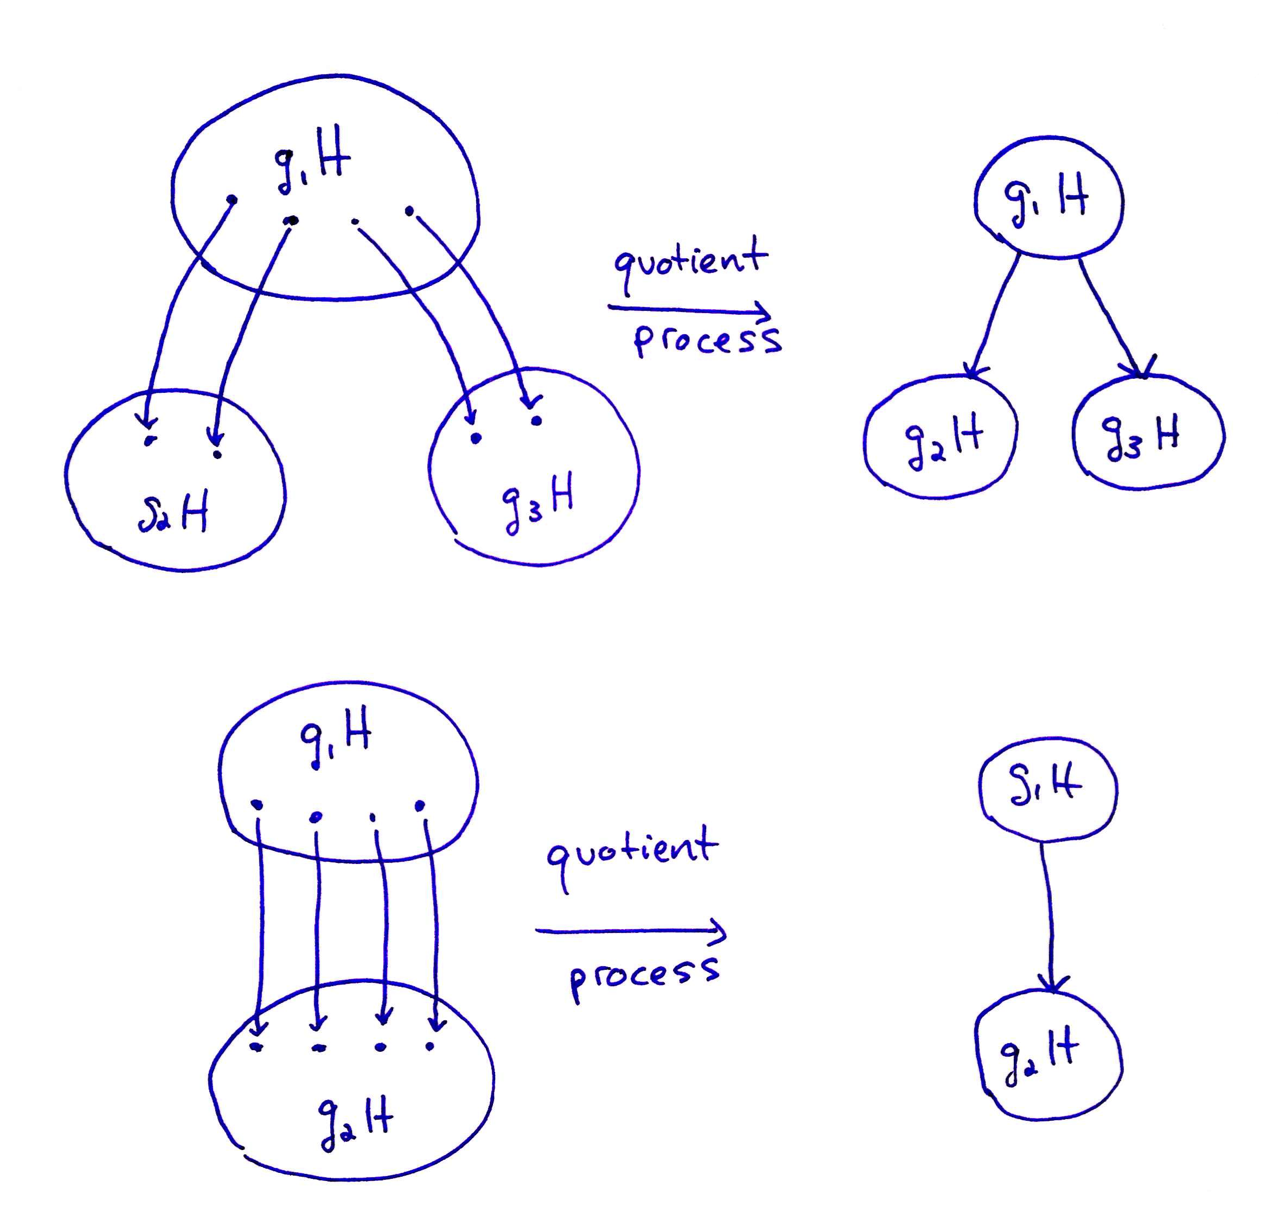
\includegraphics[width=5in]{QuotientProcess.png}
\end{center}

\begin{exercise}
In Exercise~\ref{exer:normal_in_D3}, we learned that the subgroup $K=\langle r\rangle$ is normal in $D_3$ since the left cosets are equal to the right cosets.  Note that this follows immediately from Theorem~\ref{thm:index2} since $[D_3:H]=2$.  Draw the diagram that results from performing the quotient process to $D_3$ using the subgroup $H$.  Does the resulting diagram represent a group?  If so, what group is it isomorphic to?
\end{exercise}

Now, suppose $G$ is an arbitrary group and let $H\leq G$. Consider the set of left cosets of $H$.  We define
\[
(aH)(bH):=(ab)H.
\]
The natural question to ask is whether this operation is well-defined.  That is, does the result of multiplying two left cosets depend on our choice of representative?  More specifically, suppose $c\in aH$ and $d\in bH$.  Then $cH=aH$ and $dH=bH$.  According to the operation defined above, $(cH)(dH)=cdH$.  It better be the case that $cdH=abH$, otherwise the operation is not well-defined.

\begin{exercise}
Let $H=\langle s\rangle \leq D_3$.  Find specific examples of $a,b,c,d\in D_3$ such that $(aH)(bH)\neq (cH)(dH)$.
\end{exercise}

\begin{theorem}
Let $G$ be a group and let $H\leq G$.  Then left coset multiplication (as defined above) is well-defined if and only if $H\trianglelefteq G$.
\end{theorem}

\begin{theorem}\label{thm:quotient_grp}
Let $G$ be a group and let $H\trianglelefteq G$.  Then the set of left cosets of $H$ in $G$ forms a group under left coset multiplication.
\end{theorem}

The group from Theorem~\ref{thm:quotient_grp} is denoted by $G/H$, read ``$G$ mod $H$", and is referred to the \textbf{quotient group} (or \textbf{factor group}) of $G$ by $H$.  If $G$ is a finite group, then $G/H$ is exactly the group that arises from ``gluing together" the colored blocks in a checkerboard-patterned group table.  It's also the group that we get after applying the quotient process to the Cayley diagram.  It's important to point out once more that this only works properly if $H$ is a normal subgroup.

\begin{theorem}
Let $G$ be a group and let $H\trianglelefteq G$.  Then $|G/H|=[G:H]$.  In particular, if $G$ is finite, then $|G/H|=|G|/|H|$.
\end{theorem}

\begin{exercise}%Borrowing from Fraleigh Exercises 9--15 in Section 14.
Find the order of the given element in the quotient group. You may assume that we are taking the quotient by a normal subgroup. 
\begin{enumerate}
\item[(a)] $s\langle r\rangle \in D_4/\langle r\rangle$
\item[(b)] $j\langle -1\rangle \in Q_8/\langle -1\rangle$
\item[(c)] $5+\langle 4\rangle \in \mathbb{Z}_{12}/\langle 4\rangle$
\item[(d)] $(2,1)+\langle (1,1)\rangle \in (\mathbb{Z}_3\times \mathbb{Z}_6)/\langle (1,1)\rangle$ 
\end{enumerate}
 
\end{exercise}


\begin{exercise}
For each quotient group below, describe the group.  If possible, state what group each is isomorphic to.  You may assume that we are taking the quotient by a normal subgroup. 
\begin{enumerate}
\item[(a)] $Q_8/\langle -1\rangle$
\item[(b)] $Q_8/\langle i\rangle$
\item[(c)] $\mathbb{Z}_4/\langle 2\rangle$
\item[(d)] $V_4/\langle h\rangle$
\item[(e)] $A_4/\langle (1,2)(3,4),(1,3)(2,4)\rangle$
\item[(f)] $(\mathbb{Z}_2\times \mathbb{Z}_2)/\langle (1,1)\rangle$
\item[(f)] $\mathbb{Z}/4\mathbb{Z}$
\item[(h)] $S_4/A_4$
\item[(i)] $(\mathbb{Z}_4\times \mathbb{Z}_2)/(\{0\}\times \mathbb{Z}_2)$
\end{enumerate}
\end{exercise}

\begin{theorem}
Let $G$ be a group.  Then
\begin{enumerate}
\item $G/\{e\}\cong G$
\item $G/G\cong \{e\}$
\end{enumerate}
\end{theorem}

\begin{theorem}
For all $n\in \mathbb{N}$, we have the following.
\begin{enumerate}
\item $S_n/A_n\cong \mathbb{Z}_2$ (for $n\geq 3$)
\item $\mathbb{Z}/n\mathbb{Z}\cong \mathbb{Z}_n$
\item $\mathbb{R}/n\mathbb{R}\cong \{e\}$
\end{enumerate}
\end{theorem}

\begin{theorem}
Let $G$ be a group and let $H\trianglelefteq G$.  If $G$ is abelian, then so is $G/H$.
\end{theorem}

\begin{problem}
Show that the converse of the previous theorem is not true by providing a specific counterexample.
\end{problem}

\begin{exercise}
Consider the quotient group $(\mathbb{Z}_4\times \mathbb{Z}_6)/\langle (0,1)\rangle$.
\begin{enumerate}
\item[(a)] What is the order of $(\mathbb{Z}_4\times \mathbb{Z}_6)/\langle (0,1)\rangle$?
\item[(b)] Is the group abelian?  Why?
\item[(c)] Write down all the elements of $(\mathbb{Z}_4\times \mathbb{Z}_6)/\langle (0,1)\rangle$.
\item[(d)] Does one of the elements generate the group?
\item[(e)] What well-known group is $(\mathbb{Z}_4\times \mathbb{Z}_6)/\langle (0,1)\rangle$ isomorphic to?
\end{enumerate}
\end{exercise}

\begin{theorem}
Let $G$ be a group and let $H\trianglelefteq G$.  If $G$ is cyclic, then so is $G/H$.
\end{theorem}

\begin{problem}
Show that the converse of the previous theorem is not true by providing a specific counterexample.
\end{problem}

Here are few additional exercises.  These ones are a bit tougher.

\begin{exercise}
For each quotient group below, describe the group.  If possible, state what group each is isomorphic to.  You may assume that we are taking the quotient by a normal subgroup. 
\begin{enumerate}
\item[(a)] $(\mathbb{Z}_4\times \mathbb{Z}_6)/\langle (0,2)\rangle$
\item[(b)] $(\mathbb{Z}\times \mathbb{Z})/\langle (1,1)\rangle$
\item[(c)] $S_4/\langle (1,2)(3,4),(1,3)(2,4)\rangle$
\item[(d)] $\mathbb{Q}/\langle 1\rangle$ (the operation on $\mathbb{Q}$ is addition)
\end{enumerate}
\end{exercise}

\end{section}